\chapter{Cardea}\label{sec-cardea}

\section{System Design}
Recalling related works in Chapter 2, what motivates the design of Cardea are the follow:

\begin{itemize}
\item People's privacy concerns are dependent on context. Although in certain circumstances locations are strong hints of possible privacy intrusion, generally what individuals are doing and with whom are more essential and crucial factors that directly relate to privacy.
\item People's privacy preferences vary from each other, thus they should be able to express their personal privacy preferences.
\item People's privacy preferences may change from time to time, therefore they need a way to change such preferences easily.
\end{itemize}

To achieve these objectives, we propose following solution:
\begin{itemize}
\item explain what composes context in Cardea
\item registration of privacy preferences
\item hand gesture for flexibility
\end{itemize}

\begin{table}[tb]
\centering
\caption{Scene categories.}
\label{tbl-scenecate}
\begin{tabular}{ll}
\toprule
Scene category & Scenes                                                  \\ \midrule
Eating         & banquet hall, beer garden, bistro, cafeteria,       \\
               & coffee shop, diner restaurant, food court, sushi bar  \\ \midrule
Entertainment  & ballroom, bar, discotheque, pub                         \\ \midrule
Shopping       & bazzar, clothing store, department store,             \\
               & flea market, florist shop, general store,            \\
               & gift shop, jewelry shop, market, shoe shop,              \\
               & shopping mall, supermarket                           \\ \midrule
Working        & classroom, conference, cubicle, lecture room,           \\
               & library, office, reading room                        \\ \midrule
Public places  & crosswalk, downtown, field road, forest, freeway       \\
               & park, picnic area, street                            \\ \midrule
Transportation & airplane cabin, airport, bus station, bus interior,   \\
               & subway station, train station, railroad track         \\ \midrule
Exhibition     & art gallery, museum                                  \\ \midrule
Religion       & cathedral, chapel, church, mosque, pulpit, temple     \\ \midrule
Illness        & hospital, nursing home                               \\ \midrule
Nudity         & bathroom, beach, coast, lagoon, lavatory,            \\
               & swimming pool, shower, jacuzzi                       \\ \bottomrule
\end{tabular}
\end{table}




\section{Implementation}

\subsection{Scene Classification}

\subsubsection{Data Preparing and Preprocessing}

For scene classification, we use pre-trained model of Places2 dataset provided by~\cite{links:places2mit}. In the time Cardea project was conducted, Places2 dataset provided by the authors contained 401 categories with more than 8 million training images, and the pre-trained model was based on AlexNet structure~\cite{krizhevsky2012imagenet}. By the time this thesis is writing, the dataset is deprecated and the new Places2 dataset contains 365 categories. And the authors provide more pre-trained models based on different network structures~\cite{links:places2pre}.

\begin{figure}[!htbp]
    \centering
    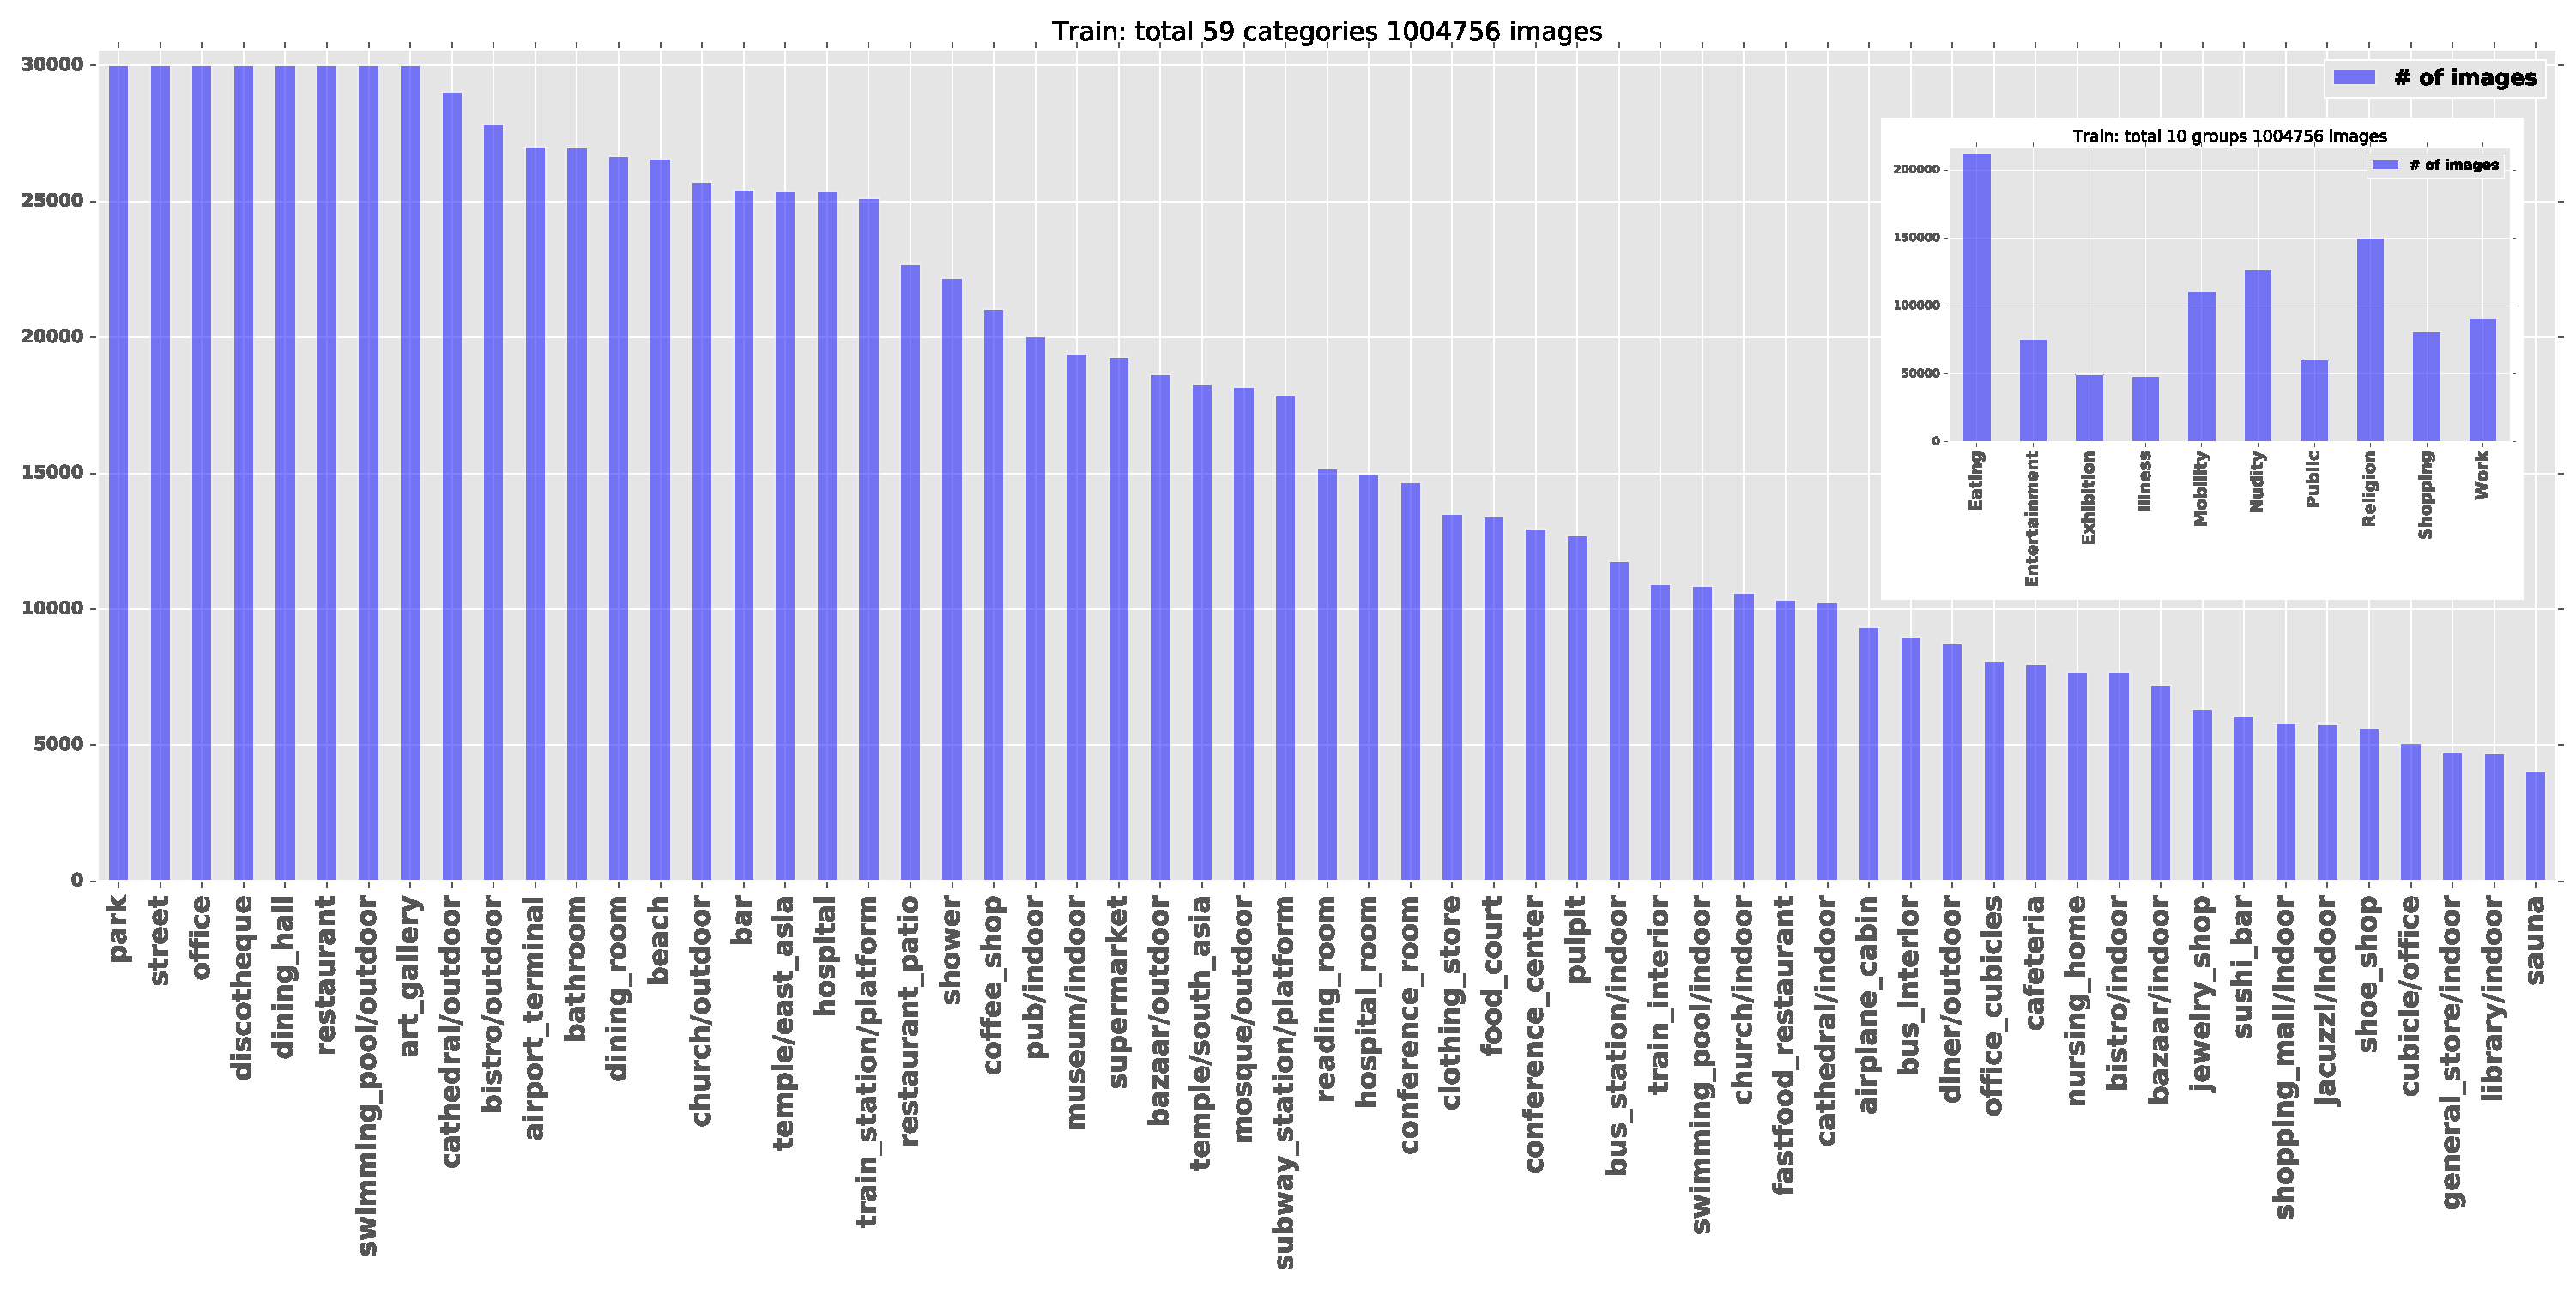
\includegraphics[width=1.0\textwidth]{figure/ch4-numdist.pdf}
    \caption{Number of images for each category and each group (inset).}
    \label{fig:ch4-scenenumdist}
\end{figure}

Note that in the dataset we used, there is a non-uniform distribution of images per category for training, ranging from 4,000 to 30,000, mimicking a more natural frequency of occurrence of the scene. Among the 401 categories, we choose 59 scene categories that are close to daily life and in such scenes people may have privacy concern. In total this subset composed of 1 million training images and 2950 validation images (50 validation images for each category). We also group these 59 scene categories into 10 groups based on contextual similarity, such that people have similar reasons for privacy in scenes that are in the same group (e.g. people don't want to be captured in bathroom and beach is both because of nudity concerns). The distribution of training images among categories and groups is shown in Fig~\ref{fig:ch4-scenenumdist}.

\subsubsection{Training Procedures}
Our training step is just a standard fine-tuning process, which is extensively used in transfer learning~\cite{sharif2014cnn,yosinski2014transferable}:

\begin{itemize}
\item[\ding{182}] Using pre-trained model as feature extractor, we extract the features at \emph{fc7} layer for images belonging to the 59 picked categories. Other than shuffling the features, we also augment the features such that all categories have same amount of features. Though the natural frequencies of occurrence are obviously different among different scenes, we argue that for the purpose of privacy protection, all the scene categories should be equally important, thus categories imbalance is not what we favored. The augmentation step can be implemented using weighted loss layer, but we take simple way of bootstrapping features for categories with less images. After this step, all features are cached and stored in lmdb format.
\item[\ding{183}] Train a softmax classifier of the 59 categories using the extracted features. We choose to train a classifier for categories and then add up the output probabilities to predict the group, rather than directly train a group classifier, is because category classifier tells more about the image, and our desired property is equal weights among scene categories rather than groups.
\item[\ding{184}] Both feature extraction and classifier training are implemented using Caffe library~\cite{links:caffelib,jia2014caffe}. In this step we merge the feature extraction part of pre-trained model and the softmax classifier into a single model by copying weights. Now Caffe has the option of specifying layers with fixed weights, thus simplifying the fine-tuning and deployment process.
\end{itemize}

Other than improving the validation accuracy from 0.56 to 0.57, shuffling also makes training converges faster. With augmentation to relieve category imbalance issue, the classifier can finally achieve 0.600 validation accuracy on the 59 categories. There is no other benchmarking result specifically on the subset we choose, but recent benchmark gives 53\%-56\% validation accuracy on the new Places2 dataset with 365 categories~\cite{links:places2pre}, suggesting our model is competitive. The higher validation accuracy of our model is due to the smaller scale of classification problem we are dealing with.

\subsubsection{Prediction}
For prediction, we get probability of a group by summing up the probabilities of all categories belonging to this group, and output the most probable group as prediction of an image. Our model's group prediction accuracy for the validation set is . Fig~\cite{} shows some prediction examples. As seen from the examples, given an image, the predicted category probabilities are usually stratified to few categories within same group, thus group prediction is resilient to perturbation of category prediction. The way we group categories can be seemed as a hard-coded clustering step, which makes prediction more robust to noise. The failure cases are mostly due to natural context ambiguity from a image (e.g. image with object in focus, therefore not enough hints for scene inference). Labeling the 342 non selected categories as extra group will amplify the ambiguity issue, even for images with less ambiguity, doing so will stratify probabilities to the extra group and lead to wrong prediction. In other words, a 59 way classifier leads to higher recall for selected scenes and grouping leads to higher accuracy.



\subsection{Face Recognition}


\subsection{Gesture Recognition}


\subsection{Deployment on Android}

\subsection{System Integration}

data flow

screen shots

decision tree



\subsection{Overview}
technical focus , final object is to prove feasibility of proposed solution, shed lights on future explorations

\section{Evaluation}


\newpage
